\chapter{Environment}
\label{chapter:environment}

In this chapter, we describe de characteristics of StarCraft II as a reinforcement learning environment followed by the modification we have made to said environment to adapt it to this project.

\section{StarCraft II}

StarCraft II is a real-time strategy video-game developed by Blizzard Entertainment, Inc in 2010. The game was extremely successful with the casual audience and it spawned a professional competition scene that continues to this day. In the field of machine learning, StarCraft II was first explored in 2017 \cite{Vinyals:2017} and it has since become a frequently tackled game thanks to its complexity and the wide range of challenges that it provides \cite{Tang:2018}.

StarCraft II is played on a mostly flat map with an isometric or birds-eye view. The main game-mode is versus, in which two or more players fight against each other until all but one of the players (or teams) are defeated. Each player needs to collect resources from the map, build structures and recruit and upgrade their army to attack other players and defend themselves. A player is defeated when all their structures have been destroyed. There are three playable races for the players to choose (Terran, Protoss and Zerg), each with their own unique units, structures, upgrade trees and game mechanics.

The game also supports user-created maps and is distributed alongside a map editor with extensive tools to create, edit and script custom maps.

\section{PySC2 library}

PySC2 is a python library developed by the Google Deep Mind team in collaboration with Blizzard \cite{Vinyals:2017}. It wraps the StarCraft II API and provides specifications for agent actions and environment observations, as well as a reward signal, which allow the use of the game as a reinforcement learning environment.

One of the major benefits of this library is that it can run the game tens of times faster than regular game-play. We can also configure how long the environment steps will be in relation to game-steps, to determine how frequently the agent will act. For example, one environment step every 16 game-steps is roughly equivalent to one action per second.

\subsubsection*{Observation}

Every step, PySC2 supplies all the information about the current state of the game, both visually and through structured data. On the visual side, the agent has access to 27 feature layers, which are pixelated RGB representations of either the game screen or the mini-map (see figure \ref{fig:feature_layers}). Each feature layer displays different aspects of the game, such as the terrain height-map, the revealed parts of the map, units of a specific type or that belong to a specific player, etc. These layers are meant to allow agents to play the game using only (or mainly) visual information similar to that which a human player would have.

Additionally, the agents also have access to structured data about the state of the game, in the form of several tensors. These tensors contain numerical information about the players, resources and units in the map, as well as accumulated data such as total damage dealt or total resources spent.

\begin{figure}[h]
    \centering
    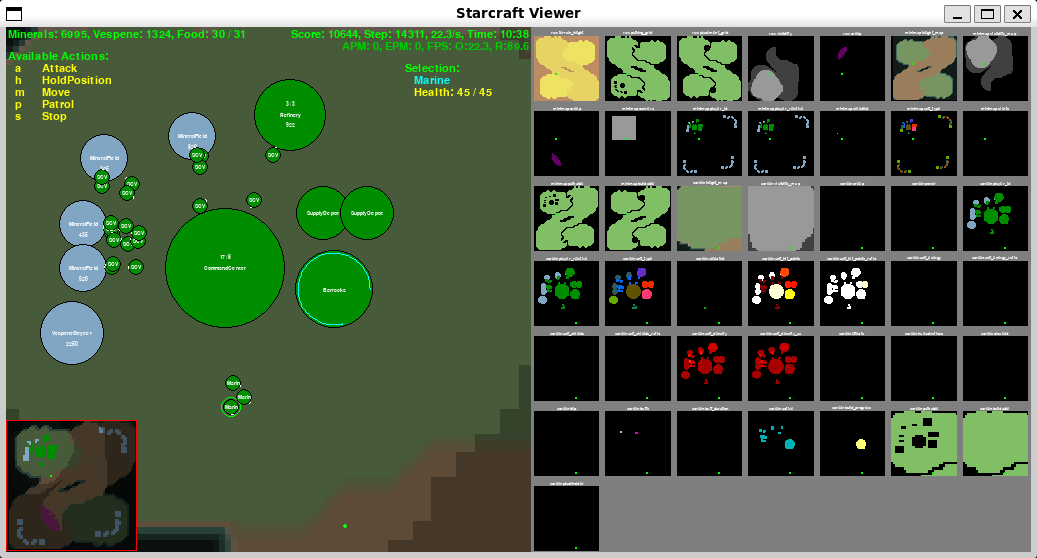
\includegraphics[width=1\textwidth]{figs/feature_layers.png}
    \caption{PySC2 feature layer view}
    \label{fig:feature_layers}
\end{figure}

\subsubsection*{Action space}

PySC2 allows the agents to interact with the game by calling functions that represent game actions that a regular player could take. These functions come in two forms. One type of function includes clicking on the screen to select a unit, dragging a rectangle to select multiple units, clicking again to issue and order to move or attack, dragging the mouse to move the camera, etc. These mimic the way the player interacts with the game, mostly by clicking the game area or the mini-map or pressing hot-keys.

The second type of function, called \say{raw functions}, encodes higher level action, such as attacking a specific point with one or more units, or building a structure. With these function, the agent doesn't need to select units before giving the command, or move the camera to be able to see the area where it wants to build. The library handles all the low level actions related to game-control and leaves the agent to focus on decision-making.

\subsubsection*{Reward signal}

For each observation in a standard versus map, PySC2 provides two different rewards. One simply reflects the win or lose status at the end of a game: 1 for victory, -1 for defeat and 0 for draw (in case of a time-out). Every step during the game before the end of the match has a reward of 0. While this reward matches the desired behavior of the agents (we simply care about winning and not losing) it can be too sparse for the agents to properly learn, since the only receive one instance of reward after every game, which can easily take hundreds or thousands of steps.

For that reason, a second, dense reward is also included. This reward matches the internal score that the game assigns to each player. This score is calculated based on the amount of resources collected, upgrades researched, and unit and structures built. It is not a perfect metric to determine victory, but it serves as a decent estimator for which player is in a better position.

\subsection{Mini-games}

PySC2 comes with a selection of mini-games, created with the StarCraft II map editor, to serve as small environments with simpler objectives. These maps often have different reward signal to better match the goal of each mini-games.

\section{Simplified environment}

Since our goal is not to create an agent as proficient as possible in the game of StarCraft II and the scope of this project is relatively modest, we have decided to simplify the environment in a way that suits our needs.

\subsection{Race selection and technology progression}

Firstly, we have limited the race selection during all of our experiments to only one of the three races. That includes for both outs agents and the opponents they will fight against. The reason for this is that all three races are extremely different in many aspects of play. They create different units and structures, follow different progressions, interact with resources in different ways and are better suited for different strategies.

Similarly, we have also decided to have the agents work with only a fraction of the entire toolset available for the race. This is because the technology progression tree of structures, units and upgrades is unnecessarily expansive and nuanced for our goals.

Taking this into account, we have chosen the Terrans as the race to focus on since it can be considered the most basic and straight-forward of the three, and the one that functions best with a limited progression. The agents will have access to the following units and structures:

\begin{itemize}
    \item \textbf{Command center:} Structure used to recruit new SCVs and necessary to collect minerals, the main resource of the game. Every player begins the game with one command center next to a patch of mineral crystals.
    \item \textbf{SCV:} Worker unit used to build all Terran structures and to collect minerals and take them to a command center. Every player begins the game with eight SCVs.
    \item \textbf{Supply depot:} Structure that increases the maximum supply of the player, which determines the amount of unit the player can have. At least one supply depot is required to build a barracks.
    \item \textbf{Barracks:} Structure used to recruit new marines.
    \item \textbf{Marine:} Ranged combat unit capable of attacking and destroying enemy units and structures.
\end{itemize}

These units, although limited for a normal game of StarCraft II, are enough for the agents to perform the basic, general steps required to win the game. The expected strategy would be:

\begin{enumerate}
    \item Gather minerals with the starting SCVs and build new SCVs to speed up the process.
    \item Optionally, build a new command center near another source of minerals and more workers to improve the resource economy.
    \item Build a supply depot.
    \item Build a barracks.
    \item Start recruiting marines while continuing to build supply depots (to allow for more marines) and barracks (to recruit marines faster).
    \item Attack the enemy base with the marines.
\end{enumerate}

\subsection{Action space}

To limit the action space to a more manageable level and to align with the limited progression described previously, we have decided on the following list of action for the agents:

\begin{itemize}
    \item \textbf{\texttt{NO\_OP:}} No action is taken for the current step.
    \item \textbf{\texttt{HARVEST\_MINERALS:}} Order a random idle worker to gather minerals from the closes mineral patch.
    \item \textbf{\texttt{BUILD\_COMMAND\_CENTER:}} Order a random idle or harvesting worker to build a command center. The agent can only have up to three command centers.
    \item \textbf{\texttt{RECRUIT\_SCV\_0:}} Recruit an SCV on the first command center.
    \item \textbf{\texttt{RECRUIT\_SCV\_1:}} Recruit an SCV on the second command center.
    \item \textbf{\texttt{RECRUIT\_SCV\_2:}} Recruit an SCV on the third command center.
    \item \textbf{\texttt{BUILD\_SUPPLY\_DEPOT:}} Order a random idle or harvesting worker to build a supply depot. The agent can only have up to 24 supply depots.
    \item \textbf{\texttt{BUILD\_BARRACKS:}} Order a random idle or harvesting worker to build a barracks. The agent can only have up to four barracks.
    \item \textbf{\texttt{RECRUIT\_MARINE:}} Recruit a marine on the barracks with the shortest queue.
    \item \textbf{\texttt{ATTACK\_CLOSEST\_BUILDING:}} Attack with all marines to the enemy building that is closest to the average position of all marines.
    \item \textbf{\texttt{ATTACK\_CLOSEST\_WORKER:}} Attack with all marines to the enemy worker that is closest to the average position of all marines.
    \item \textbf{\texttt{ATTACK\_CLOSEST\_ARMY:}} Attack with all marines to the enemy combat unit that is closest to the average position of all marines.
    \item \textbf{\texttt{ATTACK\_BUILDINGS:}} Attack with all marines to the enemy building that is closest to the average position of all enemy buildings.
    \item \textbf{\texttt{ATTACK\_WORKERS:}} Attack with all marines to the enemy worker that is closest to the average position of all enemy workers.
    \item \textbf{\texttt{ATTACK\_ARMY:}} Attack with all marines to the enemy combat unit that is closest to the average position of all enemy combat units.
\end{itemize}

For all building types, we have predefined all the position where they can be built for each map. The versus map we will use only supports up to two additional bases, which is why we limit the command centers to three (including the one each player starts with). The supply depots are limited to 24 since that is the amount that will bring the supply resource to its maximum. Any supply depot beyond the 24\textsuperscript{th} will have no effect. The limit of four barracks is somewhat arbitrary. Four is enough to build marines at a sufficient speed to win the game.

When it comes to recruiting new units, we have allowed the agent to choose in which of its command centers to build the SCVs. Because assigning too many workers to harvest on the same mineral patch has diminishing returns, and since the harvest order always points the selected worker to the closest mineral patch, this give the agent a certain amount of control on which of the bases resource economy to develop.

As for the marines, all barracks are built next to the main base and close to each other, so there is no point in differentiating between them.

\subsection{Observation}

Even though the structured observation provided by PySC2 has a predictable form, it is variable enough that it cannot be used as-is as the input for a neural network. For that reason, and for the fact that it contains considerably more information than our agent could possible need, we have created our own observation data structure to represent the state of the game. Our observation contains mostly data obtained from PySC2's observation, plus some additional data that we calculate. The complete list of fields can be found in appendix \ref{app:observation}. but some highlights include:

\begin{itemize}
    \item The amount of resourced the agent has.
    \item The number of each building type the agent has.
    \item The number of workers and marines the agent has.
    \item The number of workers that are idle, building or harvesting on each command center.
    \item The distance from the marines to various targets.
    \item The list of actions the agent can successfully take on the current step.
    \item The enemy's total army health.
\end{itemize}

\subsection{Reward signal}

The reward signals we have chosen will vary depending on the map and its objective. They are explained in detail in chapter \ref{chapter:implementation}.